\documentclass{beamer}

\usepackage[utf8]{inputenc}
\usepackage{amsmath,amssymb,tikz-cd}

\DeclareMathOperator{\im}{im}

\title{Spectral Sequences}
\author{Braden Hoagland}
\institute{Math 502: Algebraic Structures II}
\date{}

\usecolortheme{orchid}

\begin{document}

%--------------------------------------------------------------------------------
% Title Page
%--------------------------------------------------------------------------------

\begin{frame}
	\titlepage
\end{frame}

%--------------------------------------------------------------------------------
% Intro
%--------------------------------------------------------------------------------

\begin{frame}[fragile]
	\frametitle{Homology}

	\begin{itemize}
		\item Chain complex:
	\begin{equation*}
		\begin{tikzcd}
			\cdots\rar{d_{n+2}}&C_{n+1}\rar{d_{n+1}}&C_n\rar{d_n}&C_{n-1}\rar{d_{n-1}}&\cdots
		\end{tikzcd}
	\end{equation*}
	such that $d^{2}=0$.

		\item $n$-th homology: $H_{n}(A) = \ker d_n / \im d_{n+1}$.
	\end{itemize}
\end{frame}

%--------------------------------------------------------------------------------
% Preliminaries
%--------------------------------------------------------------------------------

\begin{frame}
	\frametitle{Preliminaries}

	{\color{red}Make this about motivating SS's instead.}
\end{frame}

%--------------------------------------------------------------------------------
% Filtered Complexes
%--------------------------------------------------------------------------------

\begin{frame}
	\frametitle{Filtered Complexes}

	\[
		\cdots \subset F_{p-1}C \subset F_{p}C\subset F_{p+1}C \subset \cdots
	\] 
	\begin{figure}[H]
		\centering
		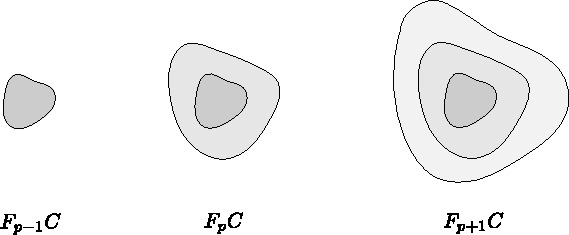
\includegraphics[scale=1]{fig/filtration.pdf}
	\end{figure}
\end{frame}

\begin{frame}[fragile]
	\frametitle{Filtered Complexes}

	Induces filtration on each element of the complex.
	\begin{overprint}
		\onslide<1>
		\[
		\begin{tikzcd}
			F_{p+1}C_{n+1}&F_{p+1}C_{n}&F_{p+1}C_{n-1}\\
			F_{p}C_{n+1}&F_{p}C_{n}&F_{p}C_{n-1}\\
			F_{p-1}C_{n+1}&F_{p-1}C_{n}&F_{p-1}C_{n-1}
		\end{tikzcd}
		\] 

		\onslide<2>
		\[
		\begin{tikzcd}
			F_{p+1}C_{n+1}\arrow[r]\arrow[dr]\arrow[ddr]&F_{p+1}C_{n}&F_{p+1}C_{n-1}\\
			F_{p}C_{n+1}&F_{p}C_{n}\rar\arrow[dr]&F_{p}C_{n-1}\\
			F_{p-1}C_{n+1}&F_{p-1}C_{n}&F_{p-1}C_{n-1}
		\end{tikzcd}
		\] 
	\end{overprint}
	\vfill

	\onslide<2> Filtered complex: $d(F_{p}C_{n}) \subset F_{p}C_{n-1}$.
\end{frame}

\begin{frame}
	\frametitle{Calculating Homology}

	\begin{itemize}
		\item Suppose calculating $H_{*}(C)$ directly is diffiult.
		\item  We can try a ``divide and conquer" strategy to make the computation easier.
	\end{itemize}
\end{frame}

\begin{frame}[fragile]
	\frametitle{Calculating Homology}

	Idea 1: Calculate the homology row by row, then sum them.
	\[
        \begin{tikzcd}
                F_{p+1}C_{n+1}\rar&F_{p+1}C_{n}\rar&F_{p+1}C_{n-1}\\
                F_{p}C_{n+1}\rar&F_{p}C_{n}\rar&F_{p}C_{n-1}\\
                F_{p-1}C_{n+1}\rar&F_{p-1}C_{n}\rar&F_{p-1}C_{n-1}
        \end{tikzcd}
        \]
	Fails because each row is a subset of the rows above it.
\end{frame}

\begin{frame}[fragile]
	\frametitle{Calculating Homology}

	Idea 2: Quotient each row by the rows below it, then calculate homology row by row and sum them.
	\[
	\begin{tikzcd}
		\frac{F_{p+1}C_{n+1}}{F_{p}C_{n+1}}\rar&\frac{F_{p+1}C_{n}}{F_{p}C_{n}}\rar&\frac{F_{p+1}C_{n-1}}{F_{p}C_{n-1}}\\
		\frac{F_{p}C_{n+1}}{F_{p-1}C_{n+1}}\rar&\frac{F_{p}C_{n}}{F_{p_1}C_{n}}\rar&\frac{F_{p}C_{n-1}}{F_{p-1}C_{n-1}}\\
		\frac{F_{p-1}C_{n+1}}{F_{p-2}C_{n+1}}\rar&\frac{F_{p-1}C_{n}}{F_{p-2}C_{n}}\rar&\frac{F_{p-1}C_{n-1}}{F_{p-2}C_{n-1}}
        \end{tikzcd}
	\] 
	{\color{white}Still fails. The rows aren't subsets of each other anymore, but $d$ still travels between rows.}
\end{frame}

\begin{frame}[fragile]
	\frametitle{Calculating Homology}

	Idea 2: Quotient each row by the rows below it, then calculate homology row by row and sum them.
	\[
		\begin{tikzcd}
			\frac{F_{p+1}C_{n+1}}{F_{p}C_{n+1}}\rar\arrow[rd]\arrow[rdd]&\frac{F_{p+1}C_{n}}{F_{p}C_{n}}&\frac{F_{p+1}C_{n-1}}{F_{p}C_{n-1}}\\
			\frac{F_{p}C_{n+1}}{F_{p-1}C_{n+1}}&\frac{F_{p}C_{n}}{F_{p_1}C_{n}}\rar\arrow[rd]&\frac{F_{p}C_{n-1}}{F_{p-1}C_{n-1}}\\
			\frac{F_{p-1}C_{n+1}}{F_{p-2}C_{n+1}}&\frac{F_{p-1}C_{n}}{F_{p-2}C_{n}}&\frac{F_{p-1}C_{n-1}}{F_{p-2}C_{n-1}}
		\end{tikzcd}
        \]

	Still fails. The rows aren't subsets of each other anymore, but $d$ still travels between rows.
\end{frame}

\begin{frame}
	{\color{red}Construct sequence and show intuition behind ``convergence"}
\end{frame}

%--------------------------------------------------------------------------------
% Convergence
%--------------------------------------------------------------------------------

\begin{frame}
	\frametitle{Convergence}

	\begin{definition}
		A spectral sequence $\left\{ E^{r} \right\}_{r \geq 0}$ \textit{converges} to a graded module $H$ if there is a filtration $F$ on $H$ such that
		\[
		E^{\infty}_{n,p} \cong F_{p}H_{n}/F_{p-1}H_{n}.
		\] 
	\end{definition}
\end{frame}

\setbeamercolor{block title}{use=structure,fg=white,bg=green!75!black}

\begin{frame}
	\frametitle{Convergence}

	\begin{theorem}
		The spectral sequence induced by a filtered complex $C$ with bounded filtration converges to $H_{*}(C)$.
	\end{theorem}

	\vspace{5mm}

	Since each column in our grid is finite, our earlier process eventually terminates.
\end{frame}

%--------------------------------------------------------------------------------
% Indexing Convention
%--------------------------------------------------------------------------------

\begin{frame}
	\frametitle{Indexing Convention}

	Most authors use a different indexing notation. Instead of
	\[
	E_{n,p}^{0} = F_{p}C_{n} / F_{p-1}C_{n},
	\] we could use complimentary degrees instead:
	\[
	E_{p,q}^{0} = F_{p}C_{p+q} / F_{p-1}C_{p+q}.
	\] 
\end{frame}

\begin{frame}[fragile]
	\frametitle{Indexing Convention}

	So instead of
	\[
	\begin{tikzcd}
		C_{n+1,p}&C_{n,p}\rar{d^{0}}\arrow[rd,"d^{1}"]\arrow[rdd,"d^{2}"]\arrow[rddd,"d^{3}"']&E_{n-1,p}\\
		C_{n+1,p-1}&C_{n,p-1}&C_{n-1,p-1}\\
		C_{n+1,p-2}&C_{n,p-2}&C_{n-1,p-2}\\
		C_{n+1,p-3}&C_{n,p-3}&C_{n-1,p-3}
	\end{tikzcd}
	\] 
\end{frame}

\begin{frame}[fragile]
	\frametitle{Indexing Convention}

	We have
	\[
	\begin{tikzcd}
		C_{p-3,q+2} & C_{p-2,q+2} & C_{p-1,q+2} & C_{p,q+2} \\
		C_{p-3,q+1} & C_{p-2,q+1} & C_{p-1,q+1} & C_{p,q+1} & \\
		C_{p-3,q} & C_{p-2,q} & C_{p-1,q} & C_{p,q}\dar{d^{0}}\lar{d^{1}}\arrow[llu,"d^{2}"]\arrow[llluu,"d^{3}"'] \\
		C_{p-3,q-1} & C_{p-2,q-1} & C_{p-1,q-1} & C_{p,q-1}
	\end{tikzcd}
	\] 
	{\color{red}Change color of the $d^{i}$.}
\end{frame}

%--------------------------------------------------------------------------------
% Final Definition
%--------------------------------------------------------------------------------

\begin{frame}
	\frametitle{Homological Spectral Sequences}

	{\color{red}Define Homological SS's based on this new bidegree.}
\end{frame}

\begin{frame}
	{\color{red}Do example about Bockstein SS.}
\end{frame}



\end{document}
